\documentclass[../TDE4-E5.tex]{subfiles}%

\begin{document}
\section[s]"2"{Oscillateur à deux ressorts}

\enonce{%
	Un mobile supposé ponctuel de masse $m$ est astreint à glisser le long d'une
	tige horizontale de direction $(Ox)$. Ce mobile est relié par deux ressort
	linéaires à deux points fixes $A$ et $B$. On le repère par sa position $\OMr =
		x$.

	\begin{center}
		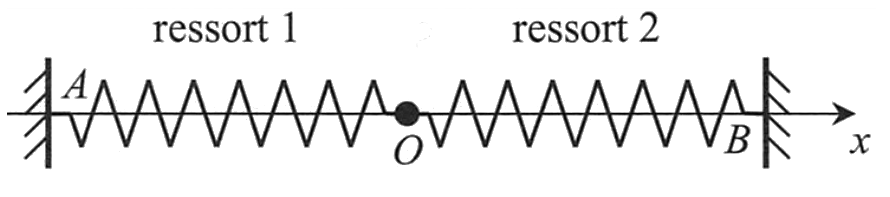
\includegraphics[width=.5\linewidth]{ressort_double}
	\end{center}

	Les deux ressorts sont identiques~: même constante de raideur $k$ et même
	longueur au repos $\ell_0$. Dans la position d'équilibre du système, les
	longueurs des ressorts sont identiques et valent $\ell_{\rm eq}$ et le mobile se
	trouve à l'origine $O$ de l'axe. On se place dans le référentiel terrestre (lié
	au sol), considérée comme galiléen. À $t = 0$, le mobile est abandonné sans
	vitesse initiale d'une position $x_0 \neq 0$
}%

\QR{%
	Dans un premier temps, on néglige tout frottement.
	\begin{enumerate}[label=\alph*)]
		\item Établir l'équation différentielle vérifiée par $x(t)$.
		\item Montrer que le système constitue un oscillateur harmonique dont on
		      précisera la pulsation $\w_0$ et la période $T_0$ propres en fonction de
		      $k$ et $m$.
		\item Donner l'expression de $x(t)$ en tenant compte des conditions
		      initiales.
	\end{enumerate}
}{%
	\begin{enumerate}[label=\alph*)]
		\item Cette fois-ci, on a deux ressorts~: le premier tire dans le sens
		      $-\ux$ et le second dans le sens $+\ux$~; ainsi le bilan des forces
		      s'exprime~:
		      \[ \begin{array}{ll}
				      \textbf{Poids}     & \Pf = -mg\uy                                      \\
				      \textbf{Support}   & \Rf = R\uy                                        \\
				      \textbf{Ressort 1} & \Ff_1 = -k(\ell_1(t) - \ell_0)\ux = -k (\ell_{\rm
				      eq} + x(t) - \ell_0)\ux                                                \\
				      \textbf{Ressort 2} & \Ff_2 = +k(\ell_2(t) - \ell_0)\ux = +k (\ell_{\rm
					      eq} - x(t) - \ell_0)\ux
			      \end{array}\]
		      On a en effet $\ell_1(t)$ la longueur du ressort 1 qui s'exprime
		      $\ell_1 = \mathrm{AM}$. Or, d'après l'énoncé $\ell_{\rm eq} =
			      \mathrm{AO} = \mathrm{OB}$~: en décomposant (\textbf{puisque les
			      distance sont sur le même axe}), on a donc $\mathrm{AM} =
			      \mathrm{AO} + \mathrm{OM} = \ell_{\rm eq} + x$.
		      \smallbreak
		      Le ressort 2 a comme longueur $\ell_2(t) =
			      \mathrm{MB} = \mathrm{MO} + \mathrm{OB}$ soit $\ell_2(t) = \ell_{\rm
				      eq} - x(t)$.
		      \smallbreak
		      Ainsi, le PFD donne
		      \begin{gather*}
			      m\af = \Pf + \Rf + \Ff_1 + \Ff_2\\
			      \Leftrightarrow m\left(
			      \begin{array}{c}
				      \dv[2]{x}{t} \\
				      0
			      \end{array}
			      \right)
			      =
			      \left(
			      \begin{array}{c}
				      -k(\bcancel{\ell_{\rm eq}} + x - \cancel{\ell_0})
				      +k(\bcancel{\ell_{\rm eq}} - x -\cancel{\ell_0}) \\
				      -mg + R
			      \end{array}
			      \right)
		      \end{gather*}
		      Sur l'axe $\ux$ on trouve
		      \begin{equation*}
			      \boxed{m \dv[2]{x}{t} + 2kx = 0} \Leftrightarrow \boxed{\dv[2]{x}{t} +
				      \frac{2k}{m}x = 0}
		      \end{equation*}
		      La projection sur $\uy$ montre que la réaction du support compense le
		      poids.
		\item Sous forme canonique, cette équation se réécrit
		      \begin{equation*}
			      \boxed{ \dv[2]{x}{t} + \w_0{}^2x = 0}
		      \end{equation*}
		      C'est bien l'équation d'un oscillateur harmonique de pulsation
		      \fbox{$\w_0 = \sqrt{\dfrac{2k}{m}}$} et donc de période \fbox{$T_0 =
				      \dfrac{2\pi}{\w_0} = 2\pi \sqrt{\dfrac{m}{2k}}$}. Doubler la
		      constante de raideur divise par $\sqrt{2}$ la période~: le ressort
		      oscille plus vite qu'avec un seul ressort.
		\item L'expression générale de $x(t)$ est donc $x(t) = A\cos(\w_0t) +
			      B\sin(\w_0t)$. Or, en $t=0$, on a $x(0) = x_0 = A$, et $ \dv{x}{t}
			      (0) = 0 = \w_0 B$~; ainsi
		      \begin{equation*}
			      \boxed{x(t) = x_0\cos(\w_0t)}
		      \end{equation*}
	\end{enumerate}
}

\QR{En fait il existe entre le mobile et la tige un frottement de type visqueux
	linéaire, la force de frottement s'exprime $\vv{F} = -\alpha\vv{v}$ (avec
	$\alpha > 0$ et $\vv{v}$ la vitesse de la masse $m$ dans le référentiel
	terrestre).
	\begin{enumerate}[label=\alph*)]
		\item Établir l'équation différentielle vérifiée par $x(t)$. On posera
		      $h = \dfrac{\alpha}{m}$.
		\item Montrer que lorsque $\alpha < 2^{3/2}\sqrt{km}$, le mouvement
		      comporte des oscillations amorties. Donner l'expression de $x(t)$ en
		      tenant compte des conditions initiales et exprimer la pseudo-période
		      $T$ en fonction de $\w_0$ et $h$.
	\end{enumerate}
}{
	\begin{enumerate}[label=\alph*)]
		\item On ajoute $\vv*{F}{\rm frott} = -\alpha v\ux$ au PFD, ce qui donne
		      \[ \boxed{ \dv[2]{x}{t} + h \dv{x}{t} + \w_0{}^2x = 0}\]
		\item On sait qu'on a des oscillations amorties quand le discriminant
		      $\Delta$ de l'équation caractéristique est négatif~: $\Delta < 0$.
		      Or ici, l'équation caractéristique est
		      \begin{gather*}
			      r^2 + hr + \w_0{}^2 = 0 \Rightarrow \Delta = h^2 - 4\w_0{}^2\\
			      \Delta < 0 \Leftrightarrow
			      \left(\frac{\alpha}{m}\right)^{\cancel{2}} <
			      \underset{2}{\cancel{4}}\w_0{}^{\cancel{2}} \Leftrightarrow \alpha < 2m
			      \sqrt{\frac{2k}{m}}\\
			      \Leftrightarrow \alpha < 2^{3/2} \sqrt{km}
		      \end{gather*}
		      Dans ce régime, on aura donc les racines
		      \begin{gather*}
			      r_\pm = - \frac{h}{2} \pm \Ir \sqrt{\w_0{}^2 - \frac{h^2}{4}}
			      \Leftrightarrow \boxed{r_\pm = - \frac{h}{2} \pm \Ir\w} \qavec
			      \boxed{\w = \sqrt{\w_0{}^2 - \frac{h^2}{4}}}
		      \end{gather*}
		      La solution générale est alors
		      \[ \boxed{x(t) = \exr^{-ht/2} \left[ D\cos(\wt) + E\sin(\wt) \right]}\]
		      On a les mêmes conditions initiales, soit $x(0) = x_0 = D$ et $
			      \dv{x}{t} (0) = 0 = - \frac{h}{2}x_0 + \w E$, d'où $E =
			      \frac{h}{2\w}x_0$. Ainsi,
		      \begin{equation*}
			      \boxed{x(t) = x_0\exr^{-ht/2} \left[ \cos(\wt) +
					      \frac{h}{2\w}\sin(\wt) \right]}
		      \end{equation*}
		      On a donc une pseudo-période \fbox{$T = \dfrac{2\pi}{\w} =
				      \dfrac{2\pi}{\sqrt{\w_0{}^2 - \frac{h^2}{4}}}$}
	\end{enumerate}
}

\end{document}
